\section{Deployment and Code Generation}
\label{sec:deploy_generate}

After the model is built, it needs to be deployed on an architecture. For the
real rover mentioned in \sect~\ref{sec:toy_rover_controller} the architecture
is a Raspberry Pi that can connect to the sensors and actuators of the device.

The virtual rover simulation environment used in the context of this article
communicates using TCP ports. Additionally, the signals flowing from the virtual
environment and back are different from the ones for the real rover. For
instance, the real rover accepts \emph{target speed} as input and the hardware
of the rover itself controls engine power (using an embedded \pid controller) in
order to attain such a speed and maintain it. The virtual rover expects that
power to the wheels is provided as a means to attain a certain speed.

\af provides a generic, non-device specific architecture for deployment, as
shown in \fig~\ref{fig:deployment_general}.

\begin{figure}[!h]
\centering
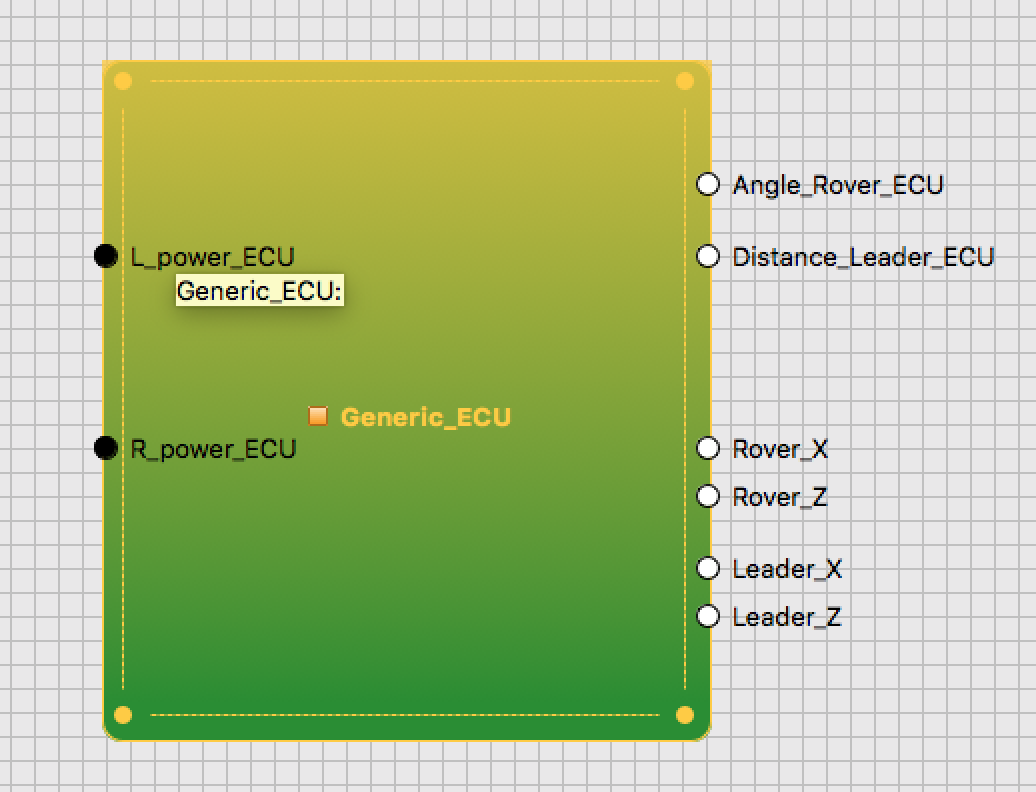
\includegraphics[width=.8\textwidth]{images/newECU.png}
\caption{A Generic ECU for the Virtual Rover Controller}
\label{fig:deployment_general}
\end{figure}

Additionally, the ports of the of the \ecu need to be mapped to the logical
ports of the controller of the model we have defined in
\sect~\ref{sec:control_vr_model}, as depicted in
figure~\ref{fig:deployment_ports}.

\begin{figure}[!h]
\centering
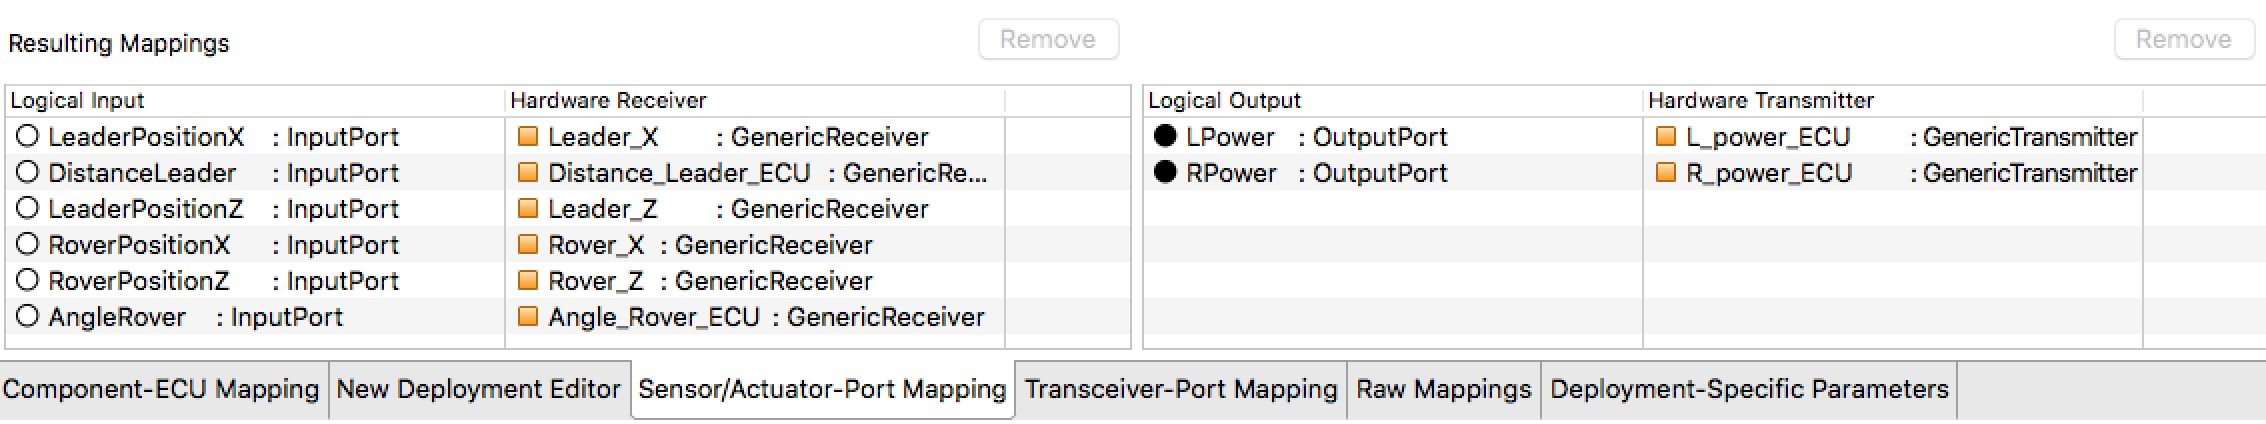
\includegraphics[width=1\textwidth]{images/newMapping.png}
\caption{Deploying the Logical Ports onto the \ecu ports}
\label{fig:deployment_ports}
\end{figure}
 
Deploying to an architecture provides the skeleton of an interface that declares
the signatures of the methods that are used by the controller logic to
communicate with the device underneath. When the architecture is fully defined,
then the glue code with the device can also be automatically generated. For our
work we have deployed onto a generic architecture as a means to automatically
generate the structure of our controller's communication infrastructure as \clang\footnote{Besides \clang, \af also allows the generating \java code.} code. The logic corresponding to the model we have presented in
\sect~\ref{sec:toy_rover_controller} is also generated as \clang code and is
meant to run in a loop with the controlled device, in this case the virtual
rover.

The \clang code that is generated for the generic architecture only provides the
interface for the functions that read the sensors and send commands on the
actuators of the virtual environment. Because of that, a manual step of
coding such methods and connecting the controller with the virtual environment
via TCP was additionally necessary to connect the controller to the rover and to
finalize the deployment of the model onto the hardware.


